\begin{statement}
    Трёхмерная сфера $S^3$ является склейкой двух полноторий.
\end{statement} 
\begin{proof}
    \[S^3 = \{x^2+y^2+a^2+b^2=1\}.\]
    Пусть 
    \[x+iy = z \in \CC,\]
    \[a+ib = w \in \CC.\]
    Тогда уравнение для сферы $S^3$ в $\CC \times \CC$ можно записать как
    \[|z|^2 + |w|^2 = 1, \ |z| \in [0,1], \ |w| \in [0,1].\]
    Если зафиксируем $|z| = z_0$, тогда удовлетворяющий уравнению сферы $|w|$ автоматически определяется как $|w| = \sqrt{1-z_0^2} = w_0$.

    Покажем, что зафиксированному модулю $z$ на сфере соответствует некоторая поверхность. По формуле Эйлера комплексные $z$ и $w$ представимы в виде 
    \[z = z_0 e^{i\phi}, \ w = w_0 e^{i\phi}.\]

    Пусть $z_0 = \frac{1}{\sqrt2}$. Определим множества 
    \[A = \{|z| \leqslant z_0\},\]
    \[B = \{|z| \geqslant z_0\}.\]
    При этом $|w| \geqslant \frac{1}{\sqrt2} = z_0$ для множества $A$ и $|w| \leqslant z_0$ для множества $B$. Они определяются симметрично и оба являются трёхмерными поверхностями с краем. Попробуем их представить.

    Рассмотрим, чему гомеоморфно $A$. $\{|z| \leqslant z_0\}$ — двумерный диск радиуса $\frac{1}{\sqrt2}$. Если выберем какую-то точку $z$ внутри диска, мы зафиксируем $|z|$ и этой точке будет соответствовать целая окружность точек вида $w$. Действительно, мы сможем однозначно определить модуль точек $w$ из модуля произвольной точки $z = \tilde{z}$ по формуле $|w| = \sqrt{1-|\tilde{z}|^2}$, тогда точки $w$ определяются как $$w = \sqrt{1-|\tilde{z}|^2} e^{i\psi}, \ \psi \in [0,2\pi],$$
    но мы не знаем угол $\psi$ этих точек $w$. То есть, угол может быть произвольным.

    Получается, что множество $A$ является декартовым произведением двумерного диска $D^2$ на окружность $S^1$, что является полноторием. Аналогично можно показать, что множество $B$ также является полноторием. Только в этом случае теперь $w$ определяют точки с двумерного диска. Следовательно, трёхмерная сфера $S^3$ является результатом склейки двух полноторий по общему граничному тору, который соответствует точкам 
    \[|z| = |w| = \frac{1}{\sqrt2}.\]

    Так как в общем случае есть несколько способов склеить два полнотория по общей границе, и не все их этих склеек эквивалентны трёхмерной сфере $S^3$. Поэтому важно рассмотреть, как именно склеиваются полнотория в нашей задаче и будет ли их склейка гомеоморфна $S^3$.

    На полнотории $A$ рассмотрим кривую
    \[|z| = \frac{1}{\sqrt2}, \ w = \frac{1}{\sqrt2}.\]
    Такая кривая стягивается в точку внутри полнотория $A$, если уменьшать $|z|$ к нулю, то есть к центру диска. $w$ при этом будет расти к единице. Внутри полнотория $B$ в качестве аналогичной стягивающейся в точку кривой можно взять $|w| = \frac{1}{\sqrt2}, z \ \frac{1}{\sqrt2}$.

    Эти две кривые пересекаются в точке $z = w = \frac{1}{\sqrt2}$.Более того, они обе лежат на общей для полноторий $A$ и $B$ границе. Поэтому можно обе эти кривые изобразить на одном полнотории, например, на $A$. Обозначим цикл, который стягивается в точку в полнотории $A$ через $\lambda$, а цикл, который стягивается в полнотории $B$ обозначим через $\mu$.

    То есть два полнотория $A$ и $B$ склеиваются по общему граничному тору со сменой ролей циклов: меридианы одного тора становятся параллелями на другом торе, и наоборот. Результатом такой склейки двух полноторий является трёхмерная сфера $S^3$.

    \begin{figure}[ht]
        \centering
        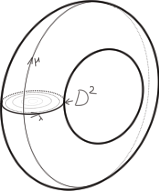
\includegraphics[scale=0.8]{images/c15.8.png}
        \caption{Циклы $\lambda$ и $\mu$ на полнотории $A$.}
        \label{fig:c15.8}
    \end{figure}
\end{proof} 


\subsection{Математический биллиард}
В нашем курсе пишем именно биллиард, а не бильярд, когда имеем в виду математический биллиард.
\begin{definition}
    \textit{Математический биллиард} — механическая система, описывающая движение материальной точки в некоторой биллиардной области $\Omega \subset \R^2$ с границей $\partial \Omega$, которая является замкнутой кривой, и упругими отражениями от границы.
\end{definition} 

\begin{remark}
    Траектория биллиарда в области определяется начальным положением точки и начальным вектором её скорости.
\end{remark}

% \begin{remark}
%     В данной системе мы пренебрегаем трением, поэтому можно считать, что абсолютное значение скорости постоянно, поэтому в момент времени $t=0$ вектор скорости можно считать единичным.
% \end{remark}

\begin{remark}
    Отражение от границы происходит по закону абсолютно упругого отражения, то есть «угол падения равен углу отражения».
\end{remark}

\begin{definition}
    \textit{Фазовое пространство системы} — множество точек 
    $$M^4(x,y,v_1,v_2) / \sim,$$
    где $x,y \in \Omega$, $v_1^2+v_2^2 > 0.$
\end{definition} 

\begin{figure}[ht]
    \centering
    \incfig[0.5\textwidth]{c15.1}
    \caption{Математический биллиард.}
    \label{fig:c15.1}
\end{figure}


Пусть $v = (v_1,v_2)$ — вектор скорости до удара, $w = (w_1,w_2)$ — вектор скорости после удара, $e = (e_1,e_2)$ — касательный вектор. Зададим отношение эквивалентности, склеивающее векторы скорости до и после удара о границу $\partial \Omega$:
\[(x,y,v_1,v_2) \sim (a,b,w_1,w_2) \Longleftrightarrow (x,y) = (a,b) \in \gamma = \partial \Omega.\]
Тогда
\[v_1^2 + v_2^2 = w_1^2 + w_2^2,\]
\[e_1v_1 + e_2v_2 = e_1w_1 + e_2w_2.\]
\begin{figure}[ht]
    \centering
    \incfig[0.5\textwidth]{c15.2}
    \caption{Биллиардный закон.}
    \label{fig:c15.2}
\end{figure}

Что произойдёт с траекторией движения материальной точки, если задать ей не скорость $(v_1,v_2)$, а, например, $(2v_1, 2v_2)$? Понятно, что траектория не изменится, просто материальная точка пройдёт её в два раза быстрее. Тогда введём следующее определение:

\begin{definition}
    \textit{Изоэнергетическая поверхность} (поверхность, на которой энергия постоянна) $Q_h^3$ — множество точек 
    \[(x,y,v_1,v_2) \in M^4\]
    таких, что 
    \[v_1^2+v_2^2 = h^2 > 0.\]
\end{definition} 

\begin{remark}
    Без ограничения общности, если не оговорено иное, всегда $h=1$.
\end{remark}

\begin{statement}
    Если $\Omega$ гомеоморфна закрытому диску $D^2$, то $Q^3 \simeq S^3$.
\end{statement} 

\begin{statement}
    Пусть $\Omega$ гомеоморфна замкнутому цилиндру, тогда $Q \simeq S^2 \times S^1$.
\end{statement} 

Функция $H = v_1^2 + v_2^2 = 1 = const$ — функция, которая сохраняет своё значение вдоль траектории биллиарда. Существует ли какая-нибудь функция $F$, которая будет функционально независима с $H$ и которая тоже сохраняет своё значение вдоль траектории?

\begin{definition}
    Функции $F$ и $H$ называются \textit{функционально независимыми}, если их градиенты линейно независимы почти всюду (то есть множество точек, где они линейно независимы, имеют меру ноль).
\end{definition} 

%я устал, пошёл есть. интегрируемые биллиарды и прочее будут к вечеру.

\begin{example}(биллиард в круге).\\
    Рассмотрим область $\Omega$, которая является двумерным диском единичного радиуса, $\partial \Omega = \{x^2+y^2=1\}$. Возьмём точку внутри и рассмотрим какую-нибудь траекторию.

    \begin{figure}[ht]
        \centering
        \incfig[0.5\textwidth]{c15.3}
        \caption{Биллиард в круге.}
        \label{fig:c15.3}
    \end{figure}

    Можно заметить несколько \textit{интегралов}: угол падения, длина хорды, расстояние от центра до хорды.

    Если расстояние от центра окружности до хорд одинаково, то можно провести окружность, радиус которой равен этому расстоянию. Такая кривая внутри биллиардной области, которая касается всех траекторий с заданным свойством, называется \textit{каустикой}.
\end{example}

\begin{definition}
    \textit{Интегрируемый биллиард} — это биллиард, вдоль траектории которого какая-то функция $F$ (кроме функции $H$) сохраняет своё значение.
\end{definition} 

Так как в определении математического биллиарда мы не ограничивали себя регулярностью кривой, то можно рассмотреть, например, биллиард в прямоугольнике.
\begin{example}(биллиард в прямоугольнике).\\
    Хоть каустики для данного биллиарда нет, но он всё равно интегрируем: звенья любой траектории лежат на прямых, принадлежащих одному из двух семейств параллельных прямых. Будет сохраняться угол между прямой, содержащей звено траектории и фиксированной прямой (например, на которой лежит сторона биллиарда) — в нашем случае это будет горизонтальная прямая.

    Тогда $\alpha$ может принимать значения из отрезка $[0, \frac{\pi}{2}]$. Граничные значения отрезка соответствуют движению точки параллельно горизонтальным или вертикальным границам прямоугольника. Обозначим отображение
    \[A: Q^3 \to \left[0, \frac{\pi}{2}\right].\]

    \begin{figure}[ht]
        \centering
        \incfig[0.5\textwidth]{c15.4}
        \caption{Биллиард в прямоугольнике.}
        \label{fig:c15.4}
    \end{figure}

    \begin{figure}[ht]
        \centering
        \incfig[0.5\textwidth]{c15.5}
        \caption{Прямоугольники, соответствующие прообразу $A^{-1}(0).$}
        \label{fig:c15.5}
    \end{figure}

    Для бильярда в прямоугольнике рассмотрим прообраз граничных значений отрезка $A^{-1}(0)$ и $A^{-1}(\frac{\pi}{2})$ в $Q^3$. Прообразом $A^{-1}(0)$ являются два прямоугольника: в одном вектора направлены вправо, в другом — влево. Эти четырёхугольники отождествляются по левой и правой граница, при это на верхней и нижней никаких отождествлений нет. Результатом склейки будет цилиндр, на котором векторы скоростей образуют «обмотки». Прообраз $A^{-1}(\frac{\pi}{2})$ рассматривается аналогично. Два соответствующих случая прямоугольника, соответствующие направленным вверх и вниз векторам скорости, склеиваются по верхней и нижней границе, результатом склейки снова является цилиндр.

    Рассмотрим прообраз $A^{-1}(\alpha_0)$, где $\alpha_0 \in \left(0, \frac{\pi}{2}\right)$. Для произвольной точки $(x,y)$ существует четыре вектора скорости, чтобы попасть на слой $\alpha_0$. Действительно, чтобы попасть на слой $\alpha_0$ звено траектории должно образовывать угол $\alpha_0$ с фиксированной прямой, содержащей границу биллиарда (например, с нижней границей прямоугольника). Таких прямых всего две, и вектор скорости может идти вдоль любой из них в одном из двух направлений. Занумеруем векторы $v_1, \dots, v_4$ как на рис.\ref{fig:c15.6}. Разобьём слой $A^{-1}(\alpha_0)$ на четыре прямоугольника, каждому поставим в соответствие по вектору скорости $v_i$.

    \begin{figure}[ht]
        \centering
        \incfig[\textwidth]{c15.6}
        \caption{Векторы скорости $A^{-1}(\alpha_0)$ и склейки листов, соответствующих векторам $v_1, \dots, v_4$.}
        \label{fig:c15.6}
    \end{figure}

    Полученные прямоугольники склеиваются в соответствии с биллиардным отображением. А именно, если на границе отождествляются векторы скорости $v_i$ и $v_j$, то по этой границе склеиваются и соответствующие им прямоугольники.

    На верхней границе отождествляются векторы $v_1 \sim v_2$, а также $v_3 \sim v_4$. Аналогичное верно для нижней границы прямоугольника. На обеих вертикальных границах отождествления также совпадут $v_1 \sim v_4$ и $v_2 \sim v_3$. 
    Изобразим склейки на рис.\ref{fig:c15.6}.

    \begin{figure}[ht]
        \centering
        \incfig[0.5\textwidth]{c15.7}
        \caption{Склейка прямоугольников.}
        \label{fig:c15.7}
    \end{figure}

    Данную склейку можно привести к склейке (см.рис.\ref{fig:c15.7}), соответствующей двумерному тору.
\end{example}